\documentclass{standalone}
\usepackage{tikz}
\usetikzlibrary{shapes.geometric, arrows}

\definecolor{mycolor}{RGB}{0, 153, 255}
\tikzstyle{process} = [rectangle, rounded corners,
                       minimum width=2cm, minimum height=1cm,
                       text centered, draw=black, fill=mycolor,
                       text=white, line width=0.3mm]

\tikzstyle{arrow} = [thick,->,>=stealth]

\begin{document}
    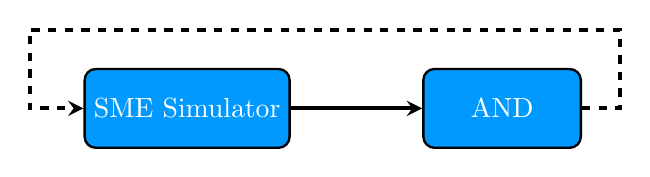
\begin{tikzpicture}[node distance=2cm]
        
        \node (Simulator) [process] {SME Simulator};
        
        \node (AND) [process, right of = Simulator, xshift=2cm] {AND};
        
        \draw [arrow, line width=0.5mm] (Simulator) -- (AND);
        
        \draw [arrow, dashed, line width=0.5mm] (AND) -- ++(1.5, 0) |- ++(0,1) |- ++(-7.5,0) |- (Simulator);
    
    \end{tikzpicture}
\end{document}
